\documentclass[10pt,a4paper]{article}
\usepackage[margin=0.82in,headheight=14pt]{geometry}
\usepackage[T1]{fontenc}
\usepackage{lmodern,microtype}
\usepackage{amsmath,amssymb}
\usepackage{booktabs,tabularx,array}
\usepackage{graphicx}
\usepackage{xcolor}
\usepackage{tikz}
\usepackage{siunitx}
\usepackage{hyperref}
\usepackage{fancyhdr}
\usepackage{caption}
\usepackage{subcaption}
\usepackage{placeins}
\usetikzlibrary{arrows.meta,decorations.pathmorphing}

\definecolor{ink}{HTML}{18313F}
\definecolor{accent}{HTML}{00677A}
\definecolor{warm}{HTML}{B44A25}
\definecolor{muted}{HTML}{52636A}
\hypersetup{colorlinks=true,linkcolor=accent,citecolor=accent,urlcolor=accent}
\sisetup{detect-all,per-mode=symbol}
\captionsetup{font=small,labelfont=bf}
\setlength{\parindent}{0pt}
\setlength{\parskip}{0.42em}
\setlength{\textfloatsep}{12pt plus 3pt minus 2pt}
\pagestyle{fancy}
\fancyhf{}
\fancyhead[L]{\small\textcolor{muted}{Advanced Control Theory}}
\fancyhead[R]{\small\textcolor{muted}{Quarter-car AFC: reproduction, diagnosis, extensions}}
\fancyfoot[C]{\thepage}

% Figures: prefer the MATLAB run (results/), fall back to the Octave reference run (results_octave/).
\newcommand{\resfig}[3][\linewidth]{\IfFileExists{results/#2/#3.pdf}{\includegraphics[width=#1,height=0.36\textheight,keepaspectratio]{results/#2/#3.pdf}}{\includegraphics[width=#1,height=0.36\textheight,keepaspectratio]{results_octave/#2/#3.pdf}}}
\newcommand{\evid}[1]{\textsc{#1}}

\title{\textbf{Approximation-Free Active Suspension Control}\large\\[0.25em]
Reproduction, diagnosis and extensions of Na et al.\ (2022)}
\author{Advanced Control Theory course project}
\date{7 October 2026}

\begin{document}
\maketitle
\vspace{-1.5em}

\begin{abstract}
Na et al.\ proposed an approximation-free control (AFC) law with prescribed performance functions (PPFs) for an electro-hydraulic quarter-car suspension and validated it on a test rig against backstepping (BSC) and PID control. We explain the method and rebuild it in five implementations that check one another: a MATLAB/Octave library, Simulink, Simscape Multibody, C running on an emulated Cortex-M4, and a browser simulator. We then test the paper's claims. Our first model, which used an assumed first-order actuator, made the paper's gains \emph{locally unstable} (spectral radius 1.02), and removing the voltage limit made it worse, so actuator saturation was a symptom rather than the cause.

On a literature electro-hydraulic plant (Alleyne--Hedrick) with two scale factors calibrated on a single paper experiment, the paper's \emph{unchanged} Case-A AFC reproduces the published indices within 7\% (IAE 0.129 vs 0.122\,m\,s) and its sub-volt control effort. BSC and PID with the paper's gains saturate, as reported, so the paper's ranking is reproduced. A hold-out test on the paper's retuned Case-B gains fails, and a joint fit generalises poorly. We conclude that the paper does not publish enough information to identify its rig, and that its gains are specific to that rig.

The control-theoretic analysis shows the following. Lemma~1 holds exactly where the valve is unsaturated. Near the origin the law is a skyhook spring of \SI{63}{kN/m}. The continuous-time closed loop is stable, but every zero-order-hold implementation is unstable through a lightly damped \SI{88}{Hz} hydraulic mode, which yields a bounded oscillation. At equal effort, LQR and skyhook match or beat AFC. On a bump, the paper's AFC chatters and lifts the wheel.

A saturation-driven envelope relaxation (our extension) removes the chatter on bumps, in a half-car as well as the quarter car. Finally, the AFC law itself costs about twice the instructions of model-based BSC on a Cortex-M4. The paper's computational advantage therefore does not come from the control law.
\end{abstract}

\noindent\textbf{Evidence labels.} \evid{Paper}: printed in Na et al.; \evid{Approx.}: read off a paper figure by eye; \evid{Calibrated}: a free factor fitted to paper data; \evid{Assumed}: not fixed by any source; \evid{Sim}: this project's output. Every number below carries one of these meanings.

\section{Research questions}
The paper asks whether a low-complexity recursive controller can keep the body displacement inside a shrinking, prescribed envelope without neural or fuzzy approximators, and whether this is practical on an electro-hydraulic rig sampled at \SI{50}{Hz} with a \(\pm\SI{5}{V}\) valve \cite{na2022}. We ask four questions:
\begin{enumerate}\itemsep0pt
\item \textbf{Method.} What exactly does AFC compute, and what does its stability proof assume?
\item \textbf{Reproduction.} Is there a physically plausible plant on which the paper's own gains reproduce its reported numbers?
\item \textbf{Validity.} Which of the paper's claims survive sampled-data analysis, robustness tests, other roads and fair comparators?
\item \textbf{Extension.} Can the failure modes we find be repaired without giving up the method's simplicity?
\end{enumerate}

\section{The paper's method}
\subsection{Plant}
\begin{figure}[!htbp]
\centering
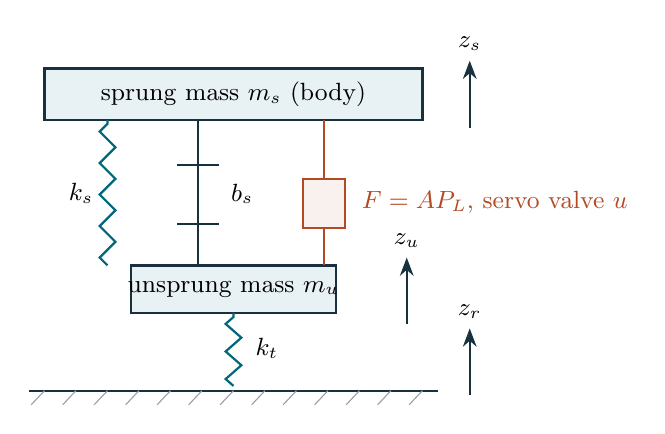
\begin{tikzpicture}[x=1cm,y=1cm,>=Stealth,thick, every node/.style={font=\small}]
  \draw[fill=accent!9,draw=ink] (1.6,3.8) rectangle (6.4,4.45);
  \node at (4,4.12) {sprung mass $m_s$ (body)};
  \draw[fill=accent!9,draw=ink] (2.7,1.35) rectangle (5.3,1.95);
  \node at (4,1.65) {unsprung mass $m_u$};
  \draw[decorate,decoration={zigzag,segment length=4mm,amplitude=1mm},draw=accent] (2.4,1.95)--(2.4,3.8);
  \node[left] at (2.35,2.87) {$k_s$};
  \draw[draw=ink] (3.55,1.95)--(3.55,2.48); \draw[draw=ink] (3.28,2.48)--(3.82,2.48);
  \draw[draw=ink] (3.55,2.48)--(3.55,3.23); \draw[draw=ink] (3.28,3.23)--(3.82,3.23);
  \draw[draw=ink] (3.55,3.23)--(3.55,3.8);
  \node[right] at (3.84,2.86) {$b_s$};
  \draw[draw=warm] (5.15,1.95)--(5.15,2.43);
  \draw[draw=warm,fill=warm!8] (4.88,2.43) rectangle (5.42,3.05);
  \draw[draw=warm] (5.15,3.05)--(5.15,3.8);
  \node[right,text=warm] at (5.5,2.75) {$F=A P_L$, servo valve $u$};
  \draw[decorate,decoration={zigzag,segment length=3.5mm,amplitude=1mm},draw=accent] (4,0.42)--(4,1.35);
  \node[right] at (4.15,0.9) {$k_t$};
  \draw[draw=ink] (1.4,0.36)--(6.6,0.36);
  \foreach \x in {1.6,2.0,...,6.4} {\draw[draw=muted!60,thin] (\x,0.36)--(\x-0.17,0.18);}
  \draw[->,draw=ink] (7.0,3.7)--(7.0,4.55) node[above] {$z_s$};
  \draw[->,draw=ink] (6.2,1.2)--(6.2,2.05) node[above] {$z_u$};
  \draw[->,draw=ink] (7.0,0.3)--(7.0,1.15) node[above] {$z_r$};
\end{tikzpicture}
\caption{Quarter car with an electro-hydraulic actuator between body and wheel. Upward is positive.}
\label{fig:mechanical}
\end{figure}
With \(d=z_s-z_u\), the mechanics are \(m_s\ddot z_s=-F_s-F_d+F\) and \(m_u\ddot z_u=F_s+F_d-F_t-F_b-F\), where \(F_s=k_sd+k_{sn}d^3\), \(F_d=b_s\dot d\) and \(F_t=k_t(z_u-z_r)\). The load pressure obeys the servo-valve law (paper eqs.~2--6):
\begin{equation}
\dot P_L=-\beta P_L-\alpha A(\dot z_s-\dot z_u)+\gamma\,x_v\sqrt{P_s-\operatorname{sgn}(x_v)P_L},\qquad \tau\dot x_v=-x_v+K_v u,\qquad |u|\le\SI{5}{V}.
\label{eq:valve}
\end{equation}
The paper sets \(\tau=0\) (\(x_v=u\)) and uses the state \(x=[z_s,\dot z_s,z_u,\dot z_u,x_5=\kappa P_L]^\mathsf T\). The constants \(\kappa\) and the valve gain are not published.

\subsection{Prescribed performance and the AFC recursion}
Each channel \(i=1,2,3\) gets an exponentially shrinking envelope and an error transformation
\begin{equation}
\mu_i(t)=(\mu_{i0}-\mu_{i\infty})e^{-\alpha_it}+\mu_{i\infty},\qquad \zeta_i=\frac{e_i}{\mu_i},\qquad \varepsilon_i=\tfrac12\ln\frac{\delta+\zeta_i}{\bar\delta-\zeta_i},
\end{equation}
and the controller is three proportional steps on the transformed errors:
\begin{equation}
e_1=x_1,\ u_1=-k_1\varepsilon_1;\qquad e_2=x_2-u_1,\ u_2=-k_2\varepsilon_2;\qquad e_3=x_5-u_2,\ u=-k_3\varepsilon_3 .
\end{equation}
Unlike backstepping, no virtual-control derivative is computed and no model term appears. Case A, used for the 10-peak road, is \(\mu_1:0.2\to\SI{0.018}{m}\) with \(\alpha_1=3\), \(\mu_2:110\to90\), \(\mu_3:100\to80\), \(\alpha_{2,3}=2\) and \(k=[25.5,12,216]\). Case B, retuned for the slower roads, is \(\mu_1:0.12\to0.018\), \(\mu_2:80\to40\), \(\mu_3:50\to20\), \(\alpha=[2,2,4]\) and \(k=[12,5,146]\). We take \(\delta=\bar\delta=1\) because the paper does not print them (\evid{Assumed}).

\subsection{What the stability proof assumes}
Lemma~1 shows that if every \(\varepsilon_i\) stays bounded then \(-\delta\mu_i<e_i<\bar\delta\mu_i\) for all \(t\) (Lemma~2: \(|\varepsilon_i|\le\varepsilon_{Mi}\Rightarrow|\zeta_i|\le\tanh\varepsilon_{Mi}<1\)). Boundedness follows from \(\dot V_i\le|\varepsilon_i|r_{Mi}(F_i-k_i c_i|\varepsilon_i|)\) with \(V_i=\varepsilon_i^2/2\). Three assumptions do the work. Time is continuous. The control input appears in \(\dot x_5\) with a known sign and \emph{without saturation}. The terms \(F_i\) are bounded on the maximal solution interval. The result is ultimate boundedness inside the funnel, not convergence to zero. Sections~\ref{sec:lyap} and \ref{sec:sampled} test each assumption.

\section{Implementations and cross-checks}
\begin{table}[!htbp]
\centering\small
\caption{Five implementations of the same equations and how they were checked against each other.}
\label{tab:impl}
\begin{tabularx}{\linewidth}{@{}>{\raggedright\arraybackslash}p{0.25\linewidth}>{\raggedright\arraybackslash}X>{\raggedright\arraybackslash}p{0.33\linewidth}@{}}
\toprule
Implementation & Role & Check\\
\midrule
\texttt{afc2} library (MATLAB R2026a; Octave 8.4 reference run) & all studies; 50\,Hz ZOH controller, RK4 plant with \SI{1}{ms} step & v1 numbers reproduced to 4 digits; MATLAB and Octave agree on every unsaturated run\\
Simulink v2 (\texttt{QuarterCar\_AFC\_v2.slx}) & editable block diagram, digital controller with sensor path & same noise, sample by sample: \(\max|\Delta z_s|=4\times10^{-16}\)\,m, \(\max|\Delta u|=2\times10^{-12}\)\,V\\
Simscape Multibody (\texttt{QuarterCar\_Multibody.slx}) & mechanics assembled from joints, not hand-written equations; \texttt{ode15s} & \(\max|\Delta z_s|=\SI{2.1}{\micro m}\); IAE 0.1294 in both\\
C (\texttt{embedded/}) & instruction counts on Cortex-M4 under QEMU & outputs equal to 10 digits\\
JavaScript web lab & interactive teaching tool & IAE equal to 4 digits\\
\bottomrule
\end{tabularx}
\end{table}

The Simulink model is the study's equations drawn as blocks: a 50\,Hz digital controller with its sensor path, a \(\pm\SI{5}{V}\) rail and the servo-valve plant (Fig.~\ref{fig:xcheck}a). Fed the same sensor noise, it reproduces the library to rounding error. The Multibody model is a stronger test, because no plant equation is copied into it. Simscape assembles the mechanics from three prismatic joints in series (road \(\to\) tyre spring \(\to\) wheel \(\to\) suspension spring, damper and actuator \(\to\) body), and only the valve law is written by hand. It matches the hand-written equations to \SI{2.1}{\micro m} over 20\,s (Fig.~\ref{fig:xcheck}b). Getting there required matching the initial state: Simscape's joints start the wheel and body moving with the road platform, while the library starts them at rest. That 11\,mm start-up discrepancy was the only one the cross-check found.

\begin{figure}[!htbp]
\centering
\begin{subfigure}{0.56\linewidth}\IfFileExists{results/phase2/simulink_v2_ideal.png}{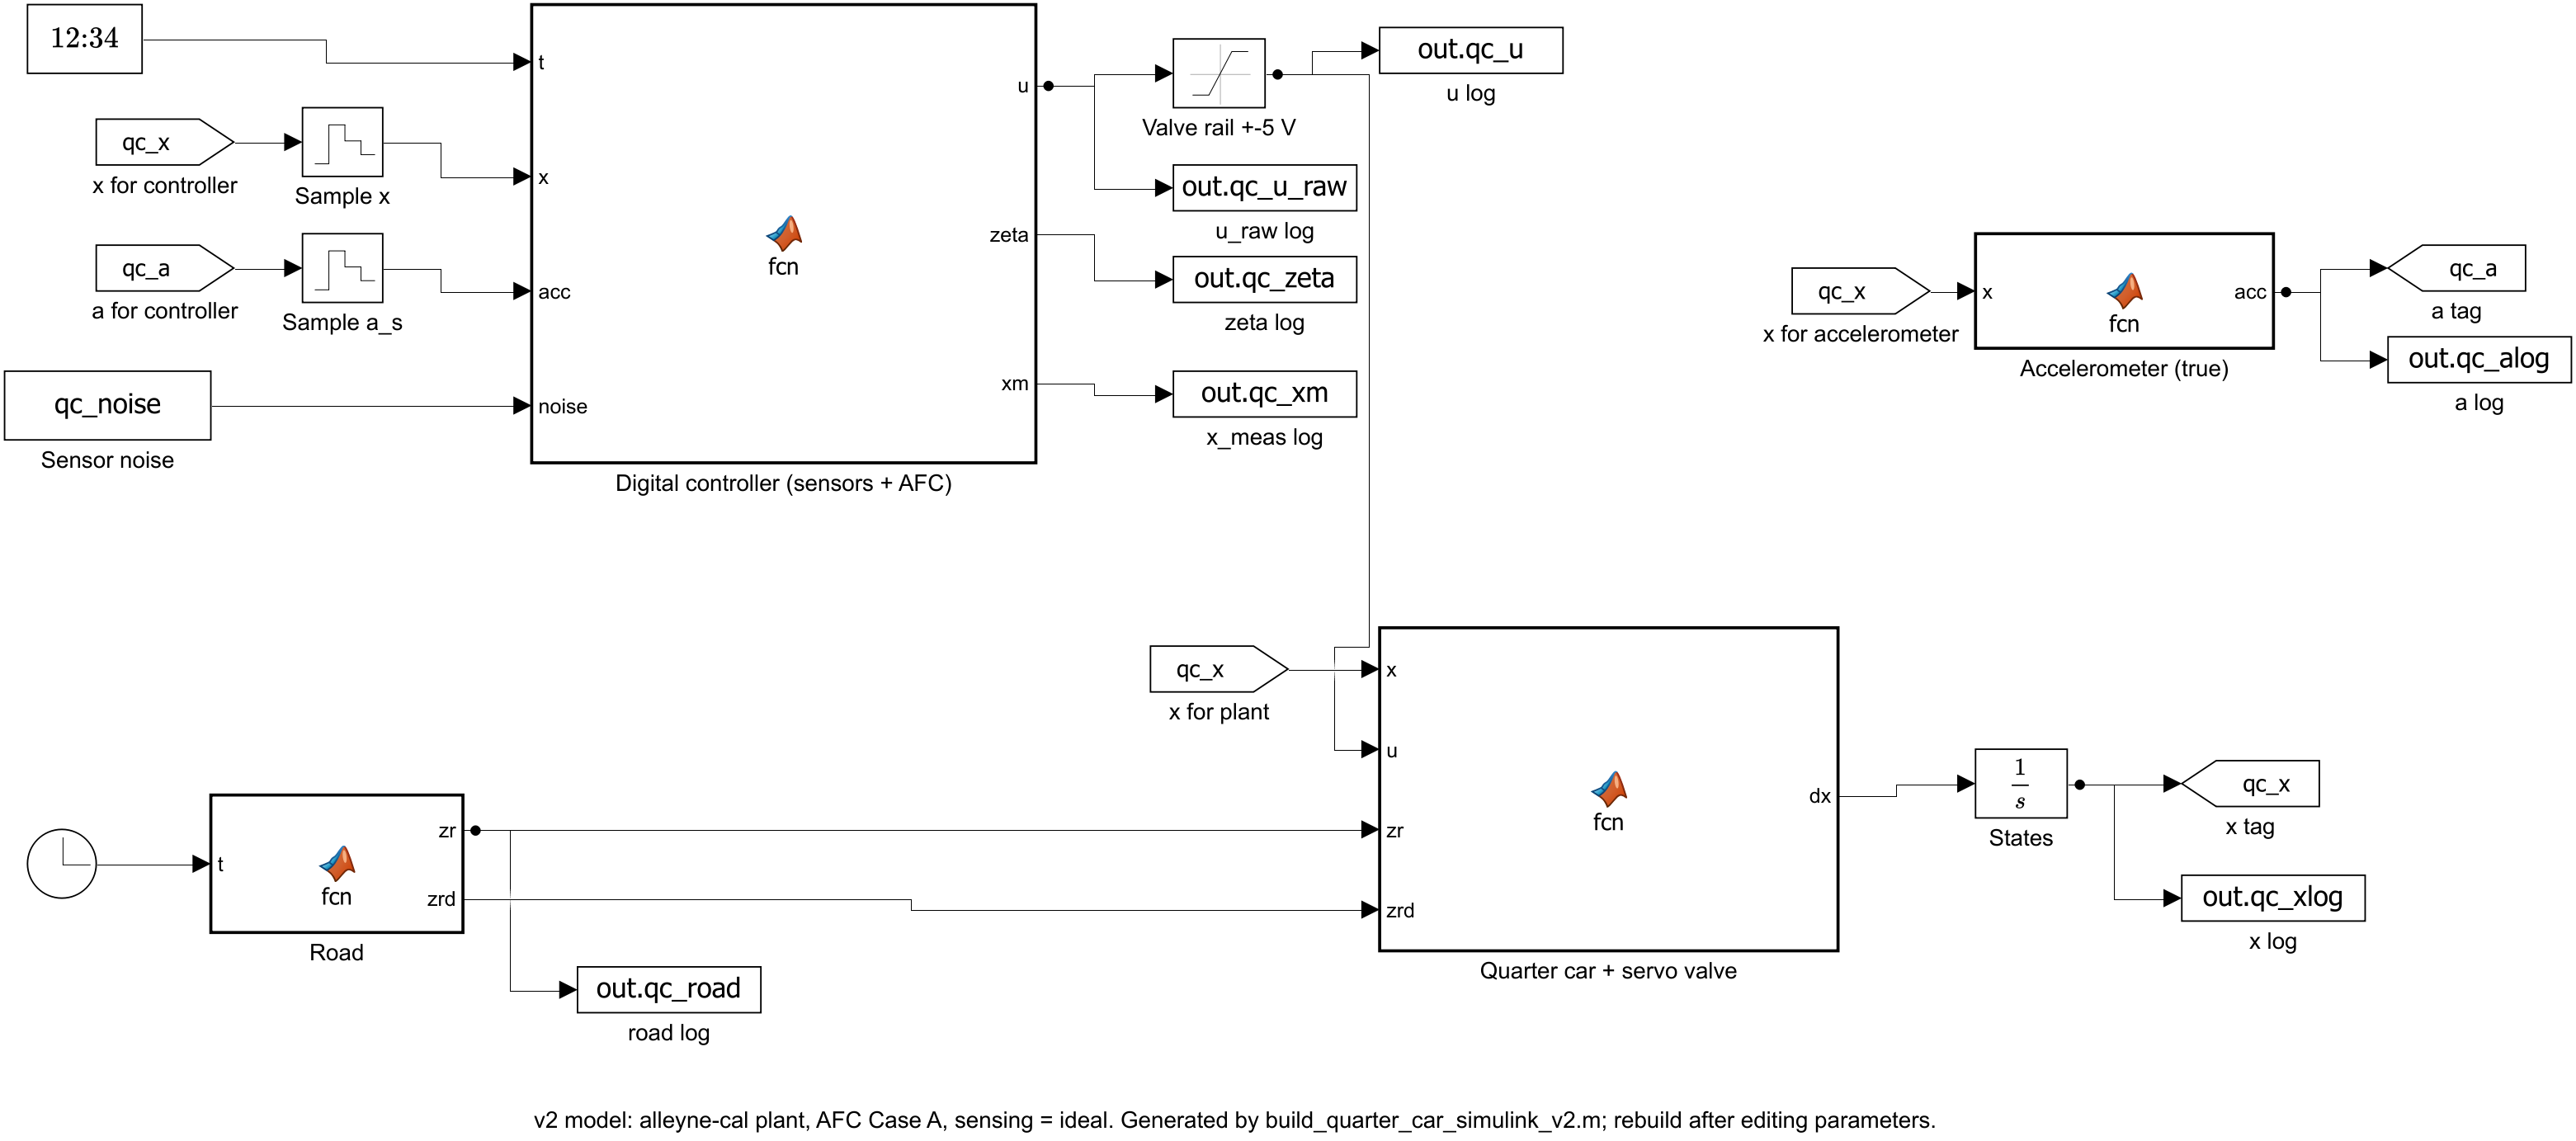
\includegraphics[width=\linewidth]{results/phase2/simulink_v2_ideal.png}}{\fbox{Simulink diagram: run run\_phase2 in MATLAB}}\caption{Simulink v2 model}\end{subfigure}\hfill
\begin{subfigure}{0.42\linewidth}\resfig{phase2b}{fig_multibody_crosscheck}\caption{Multibody vs equations, Case 10}\end{subfigure}
\caption{\evid{Sim}: two independent re-implementations of the calibrated plant with Case-A AFC.}
\label{fig:xcheck}
\end{figure}

\paragraph{Platform sensitivity.} The full study was run in MATLAB R2026a and in Octave 8.4. Every unsaturated result agrees to the printed digits. Two saturated Case-B runs do not: on the 4- and 6-peak roads AFC's IAE is 0.16 in MATLAB but 0.46--0.53 in Octave. The sampled loop is locally unstable on this plant (Sec.~\ref{sec:sampled}). When it rides the voltage rail, rounding differences between the two math libraries decide which bounded oscillation the response settles into. We report MATLAB numbers. These runs are fragile in their own right, which is one more reason the Case-B gains cannot be trusted on this plant.

\section{Baseline diagnosis: the assumed actuator}
\label{sec:v1}
Our first model (v1) used masses from Jin et al.\ \cite{jin2019} and an assumed first-order pressure state \(\dot x_5=-\beta x_5-c_{\rm rel}\dot d+b_u u\). With the paper's Case-A gains, AFC saturated in 85\% of samples and left the envelope by \SI{18.9}{mm} (\evid{Sim}). The v1 report attributed this to actuator authority. Linearising the sampled loop shows a different cause:
\begin{itemize}\itemsep0pt
\item Near the origin AFC is the static law \(u=-510\,z_s-0.36\,\dot z_s-2.70\,x_5\). On the v1 plant the 50\,Hz loop has spectral radius 1.0195, with continuous-equivalent poles at \(0.96\pm8.31j\). It is \emph{unstable}.
\item Removing the \(\pm\SI{5}{V}\) rail makes the response worse: IAE rises from 0.485 to 2.37\,m\,s and the body moves \SI{0.23}{m}. Saturation was limiting the instability, not causing it.
\item Raising or lowering the actuator gain \(b_u\) keeps the spectral radius between 0.996 and 1.68. There is no actuator size for which these gains work well on this plant (Fig.~\ref{fig:feas}, bottom).
\end{itemize}
The paper's gains are expressed in its rig's scaling (\(\kappa\), \(A\), masses). The law needs no model, but its gains do depend on the plant's scale.

\section{A literature plant calibrated to the paper}
\subsection{Model and calibration}
We use the Alleyne--Hedrick hydraulic quarter car (\(m_s=290\), \(m_u=59\)\,kg, \(k_s=16812\), \(k_t=190000\)\,N/m, \(b_s=1000\)\,N\,s/m, \(\alpha=4.515\times10^{13}\), \(\beta=1\), \(\gamma=1.545\times10^9\), \(A=3.35\times10^{-4}\)\,m\(^2\), \(P_s=10.34\)\,MPa) \cite{alleyne1995} with the full valve law~\eqref{eq:valve}. Two quantities have no published value for a voltage-driven rig: the valve gain \(K_v\) and a lumped valve/sensing lag \(\tau\). We fitted them on a \(7\times5\) grid against the paper's Case-10 AFC result: IAE, ITAE and ITSE from Fig.~7 (\evid{Paper}) and RMS voltage \(\approx\)\SI{0.5}{V} from Fig.~13 (\evid{Approx.}). The optimum is \(K_v=5\times10^{-4}\)\,m/V and \(\tau=1/30\)\,s, with a mean absolute log error of 0.042, i.e.\ about 4\% (\evid{Calibrated}). With the literature spool constant \(\tau=\SI{3}{ms}\) the best error is 0.69 (0.62 in Octave; the loop is strongly unstable there). The rig therefore behaves as if it had tens of milliseconds of lag between command and force, which matches the paper's own remark about actuator delays.

\subsection{Case 10 against the paper}
\begin{table}[!htbp]
\centering\small
\caption{Case 10 (0.043\,m, 0.505\,Hz) on the calibrated plant, all controllers with the paper's Case-A gains. \evid{Paper} values from Figs.~7 and 13 (\(^\ast\)\evid{Approx.}).}
\label{tab:case10}
\IfFileExists{results/phase1/case10_table.tex}{% Generated by run_phase1.m -- calibrated plant, paper Case A gains
\begin{tabular}{lrrrrrrrr}
\toprule
 & \multicolumn{2}{c}{IAE (m\,s)} & \multicolumn{2}{c}{ITAE (m\,s$^2$)} & \multicolumn{2}{c}{ITSE (m$^2$s$^2$)} & \multicolumn{2}{c}{$u_{\mathrm{RMS}}$ (V)}\\
Controller & sim & paper & sim & paper & sim & paper & sim & paper$^\ast$\\
\midrule
AFC & 0.1294 & 0.1216 & 1.197 & 1.140 & 0.0088 & 0.0093 & 0.50 & 0.5\\
BSC & 0.6756 & 0.2108 & 6.864 & 1.952 & 0.3101 & 0.0224 & 4.98 & 4.7\\
PID & 0.8059 & 0.1881 & 8.829 & 1.191 & 0.5517 & 0.0219 & 4.98 & 5.0\\
Passive & 0.6661 & -- & 6.651 & -- & 0.2744 & -- & 0.00 & --\\
\bottomrule
\end{tabular}
}{% Generated by run_phase1.m -- calibrated plant, paper Case A gains
\begin{tabular}{lrrrrrrrr}
\toprule
 & \multicolumn{2}{c}{IAE (m\,s)} & \multicolumn{2}{c}{ITAE (m\,s$^2$)} & \multicolumn{2}{c}{ITSE (m$^2$s$^2$)} & \multicolumn{2}{c}{$u_{\mathrm{RMS}}$ (V)}\\
Controller & sim & paper & sim & paper & sim & paper & sim & paper$^\ast$\\
\midrule
AFC & 0.1294 & 0.1216 & 1.197 & 1.140 & 0.0088 & 0.0093 & 0.50 & 0.5\\
BSC & 0.6756 & 0.2108 & 6.864 & 1.952 & 0.3101 & 0.0224 & 4.98 & 4.7\\
PID & 0.8059 & 0.1881 & 8.829 & 1.191 & 0.5517 & 0.0219 & 4.98 & 5.0\\
Passive & 0.6661 & -- & 6.651 & -- & 0.2744 & -- & 0.00 & --\\
\bottomrule
\end{tabular}
}
\end{table}
Table~\ref{tab:case10} and Fig.~\ref{fig:case10} show the result. The unchanged AFC reproduces the paper's indices within 7\%. It keeps the envelope, and its command stays below \SI{2.6}{V}, as in the paper's Fig.~10. BSC and PID with the paper's gains saturate in 99\% of samples. The paper also reports that these two saturate (Fig.~13: RMS voltage 4.7--\SI{5}{V} at 10 peaks), and AFC ranks first, as in the paper. The comparators are much worse here than on the rig (IAE 0.68/0.81 against 0.21/0.19). Their high-gain loops chatter against our plant's lag, so their absolute numbers are not transferable. The paper's measured acceleration RMS is ten times ours (1.67 vs \SI{0.17}{m/s^2}). Sensor noise explains a large part of this (Sec.~\ref{sec:sensing}).

\begin{figure}[!htbp]
\centering
\begin{subfigure}{0.49\linewidth}\resfig{phase1}{fig_case10_displacement}\caption{body displacement and envelope}\end{subfigure}\hfill
\begin{subfigure}{0.49\linewidth}\resfig{phase1}{fig_case10_control}\caption{valve command}\end{subfigure}
\caption{\evid{Sim}: Case 10 on the calibrated plant (compare paper Figs.~6 and 10).}
\label{fig:case10}
\end{figure}

\subsection{Hold-out test and identifiability}
The paper retunes AFC/BSC/PID for the seven slower roads (Case B) and reports AFC best on all eight (Fig.~12). On our plant AFC is also lowest on all eight roads. But Case-B AFC saturates for 3--9 peaks (RMS 4.1--\SI{4.4}{V} against the paper's \(\approx\)\SI{0.45}{V}), while the Case-A gains work on every road (Fig.~\ref{fig:holdout}). We then fitted \(\kappa\), \(K_v\) and \(\tau\) jointly on two training roads that use different gain sets (10/A and 6/B). The training error is 0.22 but the error on the six held-out roads is 0.63. No member of this plant family explains the rig under both gain sets. The paper does not contain enough information to identify its rig, and comparisons with it must stay at the level of trends.

\begin{figure}[!htbp]
\centering
\begin{subfigure}{0.49\linewidth}\resfig{phase1}{fig_sweep_holdout}\caption{hold-out across the eight roads}\label{fig:holdout}\end{subfigure}\hfill
\begin{subfigure}{0.49\linewidth}\resfig{phase1}{fig_feasibility}\caption{feasibility maps}\label{fig:feas}\end{subfigure}
\caption{\evid{Sim}: (a) AFC IAE and voltage per road against the paper (\evid{Approx.}); (b) envelope violation and saturation over road frequency and actuator gain, calibrated plant (top) and v1 plant (bottom).}
\end{figure}

\paragraph{Feasibility map.} On the calibrated plant, Case-A AFC keeps the envelope up to \SI{1}{Hz} for valve gains between 0.25 and 1 times the calibrated value. \emph{Doubling} the valve gain breaks it (Fig.~\ref{fig:feas}). More actuator authority is not better with fixed gains, because the inner pressure loop then becomes too fast for \SI{50}{Hz}.

\FloatBarrier
\section{Control-theoretic analysis}
\subsection{Where Lemma 1 holds}
\label{sec:lyap}
Logging \(\zeta_i\), \(\varepsilon_i\) and \(V_i=\varepsilon_i^2/2\) makes the proof's argument visible (Fig.~\ref{fig:lyap}). On the calibrated plant \(\max|\zeta_1|=0.50\) and \(\varepsilon_{M1}=0.555\). Lemma~2's bound \(|\zeta_1|\le\tanh\varepsilon_{M1}=0.504\) is tight, and the envelope holds. On the v1 plant \(\zeta\) crosses \(\pm1\) in 69.5\% of samples, and \emph{every one} of those samples is saturated. The proof's only broken assumption there is the unsaturated input. Its conclusion fails exactly where that assumption fails.

\begin{figure}[!htbp]
\centering\resfig[0.86\linewidth]{phase3}{fig_lyapunov}
\caption{\evid{Sim}: normalised errors \(\zeta_i\), transformed errors \(\varepsilon_i\) and \(V_1\); red dots mark saturated samples. Left: calibrated plant. Right: v1 plant.}
\label{fig:lyap}
\end{figure}

\subsection{AFC as a skyhook spring}
For \(|\zeta_i|\ll1\), \(\varepsilon_i\approx\zeta_i\) and the recursion collapses to \(u=-\tfrac{k_3}{\mu_3}\bigl(x_5+\tfrac{k_2}{\mu_2}(x_2+\tfrac{k_1}{\mu_1}x_1)\bigr)\). In force terms this is a pressure loop of \SI{2.7}{V} per unit \(x_5\) tracking the reference force \(F^\ast=-(A/\kappa)\tfrac{k_2}{\mu_2}\bigl(\tfrac{k_1}{\mu_1}z_s+\dot z_s\bigr)\). That is a skyhook spring of \SI{63.3}{kN/m} and a skyhook damper of only \SI{45}{N\,s/m}. As \(|z_s|\to\mu_1\) the barrier makes the spring arbitrarily stiff, which is how the bound is enforced. Fig.~\ref{fig:freq} compares the linearised transmissibility with the empirical response of the sampled nonlinear loop. At the paper's road frequency AFC reduces body motion to 0.22 of the road input, against 1.22 for passive. In the 4--8\,Hz band that the paper itself identifies as most uncomfortable, it roughly doubles the transmitted acceleration (466 against \SI{246}{s^{-2}} for passive).

\begin{figure}[!htbp]
\centering\resfig[0.82\linewidth]{phase3}{fig_frequency_response}
\caption{\evid{Sim}: road-to-body transmissibility. Lines: continuous linearisation; dots: sampled nonlinear simulation with \SI{5}{mm} sine roads.}
\label{fig:freq}
\end{figure}

\subsection{Sampled-data stability}
\label{sec:sampled}
The continuous linearised AFC loop on the calibrated plant is stable (slowest pole \(-1.71\pm15.7j\)). Every zero-order-hold implementation we tried, from 1 to \SI{20}{ms}, is unstable (spectral radius 1.03--4.4). The cause is a lightly damped hydraulic mode near \SI{88}{Hz} (\(\zeta\approx0.025\)): the half-sample delay of any ZOH removes its damping under pressure feedback. Larger lag helps (\(\rho=2.94\) at \(\tau=\SI{3}{ms}\), 1.004 at \SI{100}{ms}). In the nonlinear system the instability saturates into a bounded oscillation of \SI{0.13}{mm} at about \SI{12}{Hz} on a flat road (Fig.~\ref{fig:stab}). This is consistent with the paper's Lemma, which promises boundedness inside the envelope, and with the residual acceleration oscillations it reports. A continuous-time proof does not cover the digital implementation.

\begin{figure}[!htbp]
\centering\resfig[0.82\linewidth]{phase1}{fig_stability}
\caption{\evid{Sim}: closed-loop eigenvalues of the 50\,Hz loop, spectral radius against lag, v1 with and without the rail, and the bounded oscillation on a flat road.}
\label{fig:stab}
\end{figure}

\subsection{Effort, robustness and other roads}
\paragraph{Fair comparators.} The paper compares AFC only with BSC and PID tuned so that they saturate. Fig.~\ref{fig:trade} adds an LQR family designed on the linearised plant and a skyhook family that uses the same inner pressure loop as AFC. At AFC's effort (\SI{0.5}{V} RMS), a skyhook spring and damper reach IAE 0.086 and LQR reaches 0.071, against AFC's 0.129. Their acceleration is also lower. Scaling all AFC gains shows a narrow working window. A quarter of the paper's gains works (IAE 0.29), but half the gains saturate in 81\% of samples and twice the gains in 96\%. With half the gains the error reaches the barrier zone and the effective gain explodes; with twice the gains the inner loop is too fast for \SI{50}{Hz}. AFC's real advantages are its explicit bound and its independence from a model, not its efficiency.

\begin{figure}[!htbp]
\centering
\begin{subfigure}{0.49\linewidth}\resfig{phase3}{fig_tradeoff}\caption{displacement and comfort against effort}\label{fig:trade}\end{subfigure}\hfill
\begin{subfigure}{0.49\linewidth}\resfig{phase3}{fig_monte_carlo}\caption{Monte Carlo robustness}\label{fig:mc}\end{subfigure}
\caption{\evid{Sim}: (a) LQR and skyhook families against AFC, BSC and PID on Case 10; (b) 40 plants with \(m_s\pm15\%\), \(k_s\pm20\%\), \(b_s\pm30\%\), \(k_t\pm10\%\), \(K_v\pm30\%\) and \(\tau,\beta\times[0.5,2]\). BSC is given the exact perturbed model.}
\end{figure}

\paragraph{Robustness.} Over 40 perturbed plants (Fig.~\ref{fig:mc}), AFC keeps the envelope on 37, with a median IAE of 0.131 (range 0.115--0.533). The three failures are abrupt rather than gradual, the same cliff seen in the gain study. BSC and PID keep it on none, even though BSC is given the exact model of each plant. A pure skyhook damper also keeps it on none, because the envelope needs stiffness at low frequency, not damping.

\paragraph{Transients.} The envelope matters most on a transient, so we drive a \SI{50}{mm}, \SI{2.5}{m} bump at \SI{20}{km/h} at \(t=\SI{3}{s}\), when \(\mu_1\approx\SI{18}{mm}\) (Fig.~\ref{fig:bump}). The paper's AFC hits the barrier, saturates in 59\% of samples and switches rail to rail. The dynamic tyre load reaches 1.77 times the static load, so \emph{the wheel leaves the road}. On an ISO~8608 class-C road at \SI{54}{km/h} it saturates 89\% of the time. Skyhook and LQR handle the bump with tyre-load ratios below 0.3.

\begin{figure}[!htbp]
\centering\resfig[0.86\linewidth]{phase3}{fig_bump_iso}
\caption{\evid{Sim}: bump (left) and ISO 8608 class C (right): body displacement, acceleration and command for passive, AFC, AFC-AW, skyhook, LQR and PID.}
\label{fig:bump}
\end{figure}

\FloatBarrier
\section{Extensions}
\subsection{Saturation-aware AFC}
The failures above share one mechanism: the valve cannot deliver what the barrier demands, the error keeps growing toward the bound and the gain grows without limit. We let the envelopes breathe while the valve is saturated:
\begin{equation}
\mu_{i,\rm eff}=\mu_i(t)\,(1+\rho),\qquad \dot\rho=-\ell\rho+\gamma_\rho\frac{|u_{\rm raw}-\operatorname{sat}(u_{\rm raw})|}{V_{\max}},\qquad \ell=0.5,\ \gamma_\rho=5.
\end{equation}
The law, its simplicity and its model-free character are unchanged. On the bump, AFC-AW keeps the peak at \SI{18.8}{mm} with no saturation and a tyre-load ratio of 0.73. On Case 10 it is identical to AFC, because the valve never saturates there. On the v1 plant it trades bound tightness for smoothness (saturation 85\%\(\to\)4\%, IAE 0.48\(\to\)0.64). When the actuator cannot hold the bound, it gives the bound up gradually instead of switching rail to rail (Fig.~\ref{fig:aw}).

\subsection{Half car (paper Remark 3)}
Two calibrated corners carry a \SI{580}{kg} body with pitch inertia \SI{1100}{kg\,m^2} (\(a=1.2\), \(b=1.4\)\,m). Each corner runs the unchanged quarter-car AFC on its own body-corner states, and the rear wheel meets the road \((a+b)/v\) later. On the bump, decentralised AFC saturates 64\% of the time and raises heave acceleration from 0.39 to \SI{6.6}{m/s^2}. AFC-AW reduces this to \SI{1.3}{m/s^2} with no saturation, and a corner skyhook gives \SI{0.33}{m/s^2} (Fig.~\ref{fig:half}). The extension to full cars that the paper suggests carries over the transient weakness as well.

\begin{figure}[!htbp]
\centering
\begin{subfigure}{0.49\linewidth}\resfig{phase3}{fig_antiwindup}\caption{envelope relaxation, v1 plant}\label{fig:aw}\end{subfigure}\hfill
\begin{subfigure}{0.49\linewidth}\resfig{phase3b}{fig_halfcar_bump}\caption{half car on the bump}\label{fig:half}\end{subfigure}
\caption{\evid{Sim}: extensions.}
\end{figure}

\subsection{The paper's sensing path}
\label{sec:sensing}
The rig measures only \(z_s\) and \(\ddot z_s\). It obtains \(\dot z_s\) by integrating the accelerometer and estimates the cylinder force with an extended state observer. We reproduce this with noisy sensors (\(\sigma_z=\SI{0.5}{mm}\), \(\sigma_a=\SI{0.05}{m/s^2}\)) and a steady-state Kalman filter on the same two signals. The paper's claim that integration beats differentiation holds: the velocity error is 0.025 against \SI{0.034}{m/s} RMS. AFC barely depends on velocity, because \(\mu_2\) is large. Sensor noise does double to triple the acceleration RMS (0.17\(\to\)\SI{0.36}{m/s^2}), and at four times the nominal noise it reaches \SI{1.1}{m/s^2}, approaching the paper's measured \SI{1.67}{m/s^2}.

\subsection{Computation time (paper Table III)}
The same laws in C (outputs identical to 10 digits) were run on a Cortex-M4 without FPU, the core of the paper's MK60D, under QEMU with one virtual tick per instruction. Per call they take 18\,070 (AFC), 9\,275 (BSC) and 940 (PID) instructions, i.e.\ about 0.18--0.27, 0.09--0.14 and \SI{0.01}{ms} at \SI{100}{MHz}. The paper reports 4.2, 5.8 and \SI{2.6}{ms}. The laws account for a small fraction of those times, and the law alone makes AFC about twice as expensive as BSC because of three \(\exp\) and three \(\ln\) calls. Advancing the envelopes recursively removes the \(\exp\) calls (11\,264 instructions). The paper's computational advantage must come from other parts of its implementation.

\section{Assessment of the paper's claims}
Table~\ref{tab:claims} summarises each of the paper's claims against the evidence above.
\begin{table}[!htbp]
\centering\small
\caption{The paper's claims against this project's evidence.}\label{tab:claims}
\begin{tabularx}{\linewidth}{@{}>{\raggedright\arraybackslash}p{0.30\linewidth}X>{\raggedright\arraybackslash}p{0.13\linewidth}@{}}
\toprule
Claim (Na et al.) & Our evidence & Verdict\\
\midrule
Displacement stays inside the PPF for all \(t\) & Holds on the calibrated plant on Case 10, with Lemma 2 tight. Fails under saturation (v1), on bumps and on ISO roads, which is exactly where the proof's unsaturated-input assumption fails. & Conditional\\
AFC beats BSC and PID & Reproduced with the paper's gains, because the comparators saturate. At equal effort LQR and skyhook match or beat AFC. & Reproduced, comparison narrow\\
Smaller, smoother control signal & Reproduced (\SI{0.5}{V} RMS against \(\approx\)\SI{5}{V}). & Reproduced\\
No model needed & True of the law. The gains are tied to the rig's scaling: unstable on v1, Case B fails hold-out, and halving the gains crosses a stability cliff. & Qualified\\
Stability proof covers the implementation & Continuous-time only. The 50\,Hz loop is locally unstable and settles into a bounded oscillation. & Qualified\\
Lower computation than BSC & Not supported by law-level instruction counts. & Not supported\\
Velocity from integrated acceleration is preferable & Supported. & Reproduced\\
Extends to full cars & Works per corner, but keeps the transient weakness. Envelope relaxation fixes it. & Partly\\
\bottomrule
\end{tabularx}
\end{table}

\section{Tools and reproducibility}
A parametric FreeCAD model of the test rig (\texttt{cad/}) exports STEP/STL parts. Blender scripts animate both the schematic and the CAD rig from simulated trajectories (\texttt{animation/}, \texttt{cad/render\_rig.py}). An interactive web lab runs the same equations in the browser. Each study is one MATLAB call: \texttt{run\_phase1} (diagnosis, calibration, hold-out, feasibility, stability), \texttt{run\_phase2} (Simulink v2, sensing, timing), \texttt{run\_phase2b} (Multibody), \texttt{run\_phase3} (theory and comparators) and \texttt{run\_phase3b} (half car). Every number in this report is printed to a \texttt{*\_summary.txt} file by those scripts; the figures and numbers here come from the MATLAB R2026a run (\texttt{results/}, about four minutes for the whole study). The Octave reference run (\texttt{results\_octave/}) reproduces every unsaturated number without MATLAB.

\section{Conclusions}
AFC is a compact and elegant way to put a transient specification into a controller. Its proof explains when it works: when the actuator can deliver what the barrier asks for. With the paper's own gains we reproduced its headline numbers on a calibrated literature plant. We also found that the gains depend on the plant's scale, that the 50\,Hz implementation is locally unstable but practically bounded, that classic linear designs match it at equal effort, and that on transients the barrier drives the valve into saturation. Envelope relaxation is a one-line extension that keeps the method's simplicity and removes the worst failure mode. A quantitative replication would require the rig's identified valve gain, effective lag and pressure scaling. With those three numbers, everything above can be re-run unchanged.

\begin{thebibliography}{9}
\bibitem{na2022} J. Na, Y. Huang, X. Wu, Y.-J. Liu, Y. Li, and G. Li, ``Active Suspension Control of Quarter-Car System With Experimental Validation,'' \emph{IEEE Trans. Syst., Man, Cybern.: Syst.}, vol. 52, no. 8, pp. 4714--4726, 2022. \href{https://doi.org/10.1109/TSMC.2021.3103807}{doi:10.1109/TSMC.2021.3103807}.
\bibitem{alleyne1995} A. Alleyne and J. K. Hedrick, ``Nonlinear adaptive control of active suspensions,'' \emph{IEEE Trans. Control Syst. Technol.}, vol. 3, no. 1, pp. 94--101, 1995.
\bibitem{jin2019} P. Jin, W. Xue, and K. Li, ``Actuator Fault Estimation for Vehicle Active Suspensions Based on Adaptive Observer and Genetic Algorithm,'' \emph{Shock and Vibration}, 2019, 1783850. \href{https://doi.org/10.1155/2019/1783850}{doi:10.1155/2019/1783850}.
\bibitem{bechlioulis2014} C. P. Bechlioulis and G. A. Rovithakis, ``A low-complexity global approximation-free control scheme with prescribed performance for unknown pure feedback systems,'' \emph{Automatica}, vol. 50, no. 4, pp. 1217--1226, 2014.
\end{thebibliography}
\end{document}
